\section{АНАЛІЗ СТАНУ ФОРМУВАННЯ ІКК У ДИЗАЙН-ОСВІТІ УКРАЇНИ НА ОСНОВІ ДАНИХ}\label{sec:2}

\subsection{Загальнонаціональний аналіз 122 українських програм дизайну}\label{subsec:2.1}

Цей підрозділ представляє результати комплексного обчислювального аналізу всіх акредитованих освітніх програм спеціальності 022~Дизайн в Україні. Дані отримано шляхом систематичного скрепінгу Єдиної державної електронної бази з питань освіти (ЄДЕБО) та порталу Національного агентства із забезпечення якості вищої освіти (НАЗЯВО) з використанням спеціально розробленого програмного інструменту на базі Python/Playwright.

\subsubsection{Описова статистика}\label{sssec:2.1.1}

Проаналізовано \textbf{122 освітні програми} спеціальності 022~Дизайн, що охоплюють три рівні вищої освіти: бакалавр (74 програми, 60,7\%), магістр (43 програми, 35,2\%) та доктор філософії (5 програм, 4,1\%). Загалом ці програми містять \textbf{3\,043 освітні компоненти}, з яких 1\,515 мають унікальні назви.

\begin{table}[htbp]
\centering
\caption{Загальна характеристика вибірки програм спеціальності 022 Дизайн}\label{tab:naqa-descriptive}
\small
\begin{tabularx}{\textwidth}{@{}Xrrrr@{}}
\toprule
\textbf{Показник} & \textbf{Бакалавр} & \textbf{Магістр} & \textbf{PhD} & \textbf{Усього} \\
\midrule
Кількість програм & 74 & 43 & 5 & 122 \\
Кількість компонентів & 2\,442 & 559 & 42 & 3\,043 \\
Середня кількість дисциплін & 33,0 & 13,0 & 8,8 & 24,9 \\
Стандартне відхилення & 12,1 & 6,4 & 3,2 & 12,9 \\
Діапазон & 12--73 & 7--38 & 5--14 & 7--73 \\
Медіана & 32 & 12 & 8 & 24 \\
Частка вибіркових компонентів & $\approx$0\% & $\approx$0\% & $\approx$0\% & $\approx$0\% \\
Покриття силабусами & 99,0\% & 98,5\% & 97,6\% & 99,0\% \\
\bottomrule
\end{tabularx}
\end{table}

Структура компонентів за типами: обов'язкові~--- 2\,602 (85,5\%), практики~--- 335 (11,0\%), атестації~--- 105 (3,5\%), вибіркові~--- лише 1 ($<$0,1\%). Останній показник є критичним: фактична \textbf{відсутність вибіркових компонентів} свідчить про ригідну структуру навчальних програм дизайну в Україні, що обмежує можливості оперативного введення нових дисциплін, зокрема пов'язаних із ШІ та ІКК.

Найбільш поширені дисципліни: Практика (84 програми), Живопис (43), Рисунок (42), Філософія (40), Іноземна мова (36), Графіка (24). Домінування традиційних мистецьких та загальноосвітніх дисциплін у верхній частині рейтингу свідчить про класичну орієнтацію українських програм дизайну, де цифрові та ШІ-компоненти представлені значно слабше.

\subsubsection{Мережевий аналіз навчальних програм}\label{sssec:2.1.2}

Для дослідження структурних зв'язків між дисциплінами побудовано граф спільної зустрічальності (co-occurrence graph), де вузли~--- це дисципліни, а ребра з'єднують дисципліни, що зустрічаються в одній програмі. Характеристики мережі:

\begin{itemize}
    \item \textbf{1\,240 вузлів} (унікальних дисциплін) та \textbf{7\,524 ребер} (зв'язків);
    \item низька щільність мережі ($D = 0{,}0098$), що свідчить про значну варіативність навчальних планів;
    \item помірний коефіцієнт кластеризації ($C = 0{,}3641$), що вказує на наявність стійких тематичних груп;
    \item 732 зв'язаних компоненти, найбільший~--- 507 вузлів.
\end{itemize}

Алгоритм Лувена (Louvain community detection) виявив \textbf{10 спільнот} (community) у мережі. Аналіз їх складу розкриває тематичну структуру українських програм дизайну:

\begin{longtable}{@{}p{0.06\textwidth}p{0.06\textwidth}p{0.80\textwidth}@{}}
\caption{Спільноти у мережі навчальних програм (10 найбільших)}\label{tab:communities} \\
\hline
\textbf{№} & \textbf{Обсяг} & \textbf{Ядро спільноти (центральні дисципліни)} \\
\hline
\endfirsthead
\hline
\textbf{№} & \textbf{Обсяг} & \textbf{Ядро спільноти} \\
\hline
\endhead
1 & 69 & Практика, Графіка, Проєктна робота~--- \textit{прикладне ядро} \\
3 & 56 & Живопис, Рисунок, Дизайн/Проєктування~--- \textit{традиційне мистецьке ядро} \\
6 & 49 & Наукові дослідження, Теорія дизайну, Ергономіка~--- \textit{теоретичний кластер} \\
7 & 49 & Філософія, Іноземна мова, Українська мова~--- \textit{загальноосвітній кластер} \\
\hline
\end{longtable}

Жодна зі спільнот \textbf{не має центру у цифрових або ШІ-дисциплінах}. Це структурне спостереження підтверджує, що цифрова/ШІ-тематика не утворила самостійного кластера в українських програмах дизайну і залишається периферійною.

Найбільш центральні дисципліни за показником ступеня (degree centrality): Філософія (315 зв'язків), Живопис (247), Рисунок (225), Практика (204). Філософія має найбільшу кількість зв'язків тому, що є обов'язковим загальноосвітнім компонентом більшості програм, а не через змістову спорідненість із дизайном. Це підкреслює проблему <<завантаженості>> програм загальноосвітніми дисциплінами за рахунок фахових.

\subsubsection{Тематичне моделювання навчальних дисциплін}\label{sssec:2.1.3}

Для виявлення латентних тематичних структур у курикулумах застосовано тематичне моделювання BERTopic~\cite{Musiienko2025DesignEducation} з мультимовними ембедінгами (paraphrase-multilingual-mpnet-base-v2) та UMAP-кластеризацією. Моделювання виконано на масиві 3\,043 назв дисциплін з попереднім лематизуванням засобами spaCy (uk\_core\_news\_lg) та видаленням стоп-слів.

Алгоритм автоматично виявив \textbf{134 теми}. Десять найбільших тем (табл.~\ref{tab:topic-modeling}) охоплюють: практику та пленерний живопис (4,2\%), рисунок та ілюстрацію (2,4\%), живопис (2,3\%), кваліфікаційні роботи (2,0\%), філософію (1,9\%), проєктування об'єктів (1,7\%), українську мову (1,7\%), іноземну мову (1,5\%), проєктування (1,5\%), історію мистецтва (1,3\%).

\begin{table}[htbp]
\centering
\caption{Результати тематичного моделювання навчальних дисциплін (BERTopic, 10 найбільших тем)}\label{tab:topic-modeling}
\small
\begin{tabularx}{\textwidth}{@{}cXrr@{}}
\toprule
\textbf{Тема} & \textbf{Ключові слова} & \textbf{$N$} & \textbf{\%} \\
\midrule
0 & практика, пленер, живописний & 129 & 4,2 \\
1 & рисунок, ілюстрація, інфографіка & 73 & 2,4 \\
2 & живопис, фаховий & 71 & 2,3 \\
3 & кваліфікаційний, бакалавр, магістер & 62 & 2,0 \\
4 & філософія, студія, думка & 57 & 1,9 \\
5 & проєктування, об'єкт, взаємодія & 53 & 1,7 \\
6 & українська мова, діловий & 53 & 1,7 \\
7 & іноземна мова, професійний & 47 & 1,5 \\
8 & проєктування, комплексний, управління & 45 & 1,5 \\
9 & мистецтво, історія, музейний & 40 & 1,3 \\
\bottomrule
\end{tabularx}
\end{table}

Критичним спостереженням є те, що \textbf{жодна з 10 найбільших тем не пов'язана з цифровими технологіями або ШІ}. Тематичний ландшафт повністю визначається традиційними мистецькими дисциплінами (живопис, рисунок, пленер), загальноосвітніми компонентами (філософія, мови) та проєктною діяльністю. Аналіз розподілу тем за рівнями освіти (рис.~\ref{fig:topic-heatmap}) підтверджує цю тенденцію: бакалаврські програми мають більшу концентрацію практичних та мистецьких тем, магістерські~--- дослідницьких та проєктних, проте ШІ-тематика відсутня на всіх рівнях.

\begin{figure}[htbp]
\centering
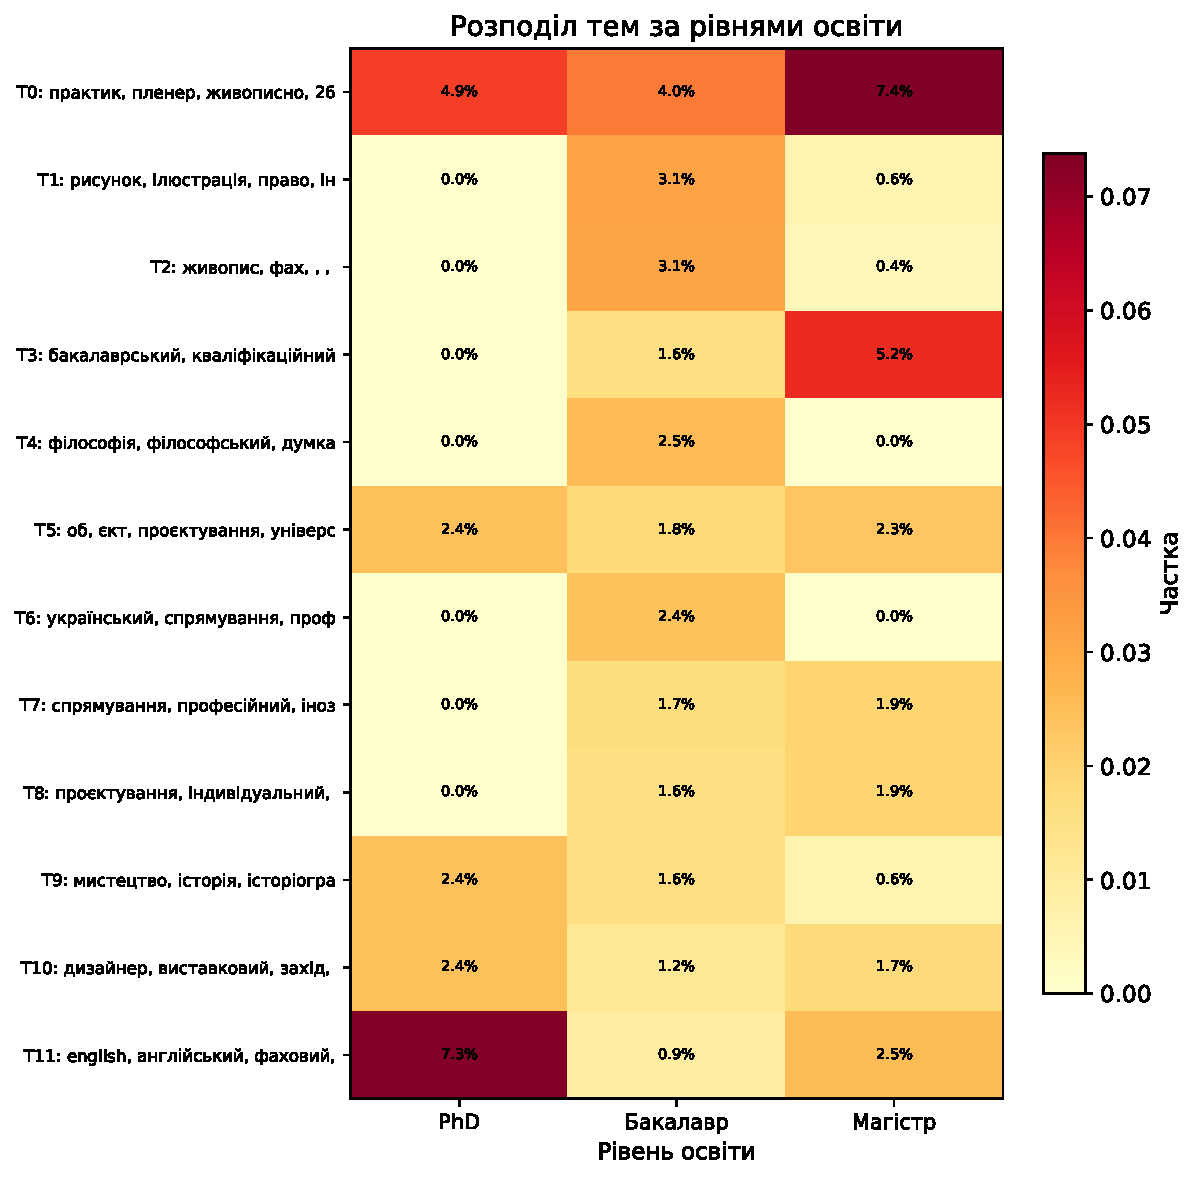
\includegraphics[width=0.75\textwidth]{figures/topic_level_heatmap.pdf}
\caption{Розподіл тем за рівнями освіти (BERTopic)}\label{fig:topic-heatmap}
\end{figure}

\subsubsection{Семантична подібність програм}\label{sssec:2.1.4}

Для дослідження структурної однорідності програм обчислено семантичну подібність між 122 програмами на основі курсових портфелів. Для кожної програми сформовано текстовий вектор шляхом конкатенації назв усіх дисциплін, після чого згенеровано ембедінги (paraphrase-multilingual-mpnet-base-v2) та обчислено матрицю косинусної подібності розмірністю $122 \times 122$.

Середня міжпрограмна подібність становить $\bar{s} = 0{,}772$ ($\sigma = 0{,}089$, діапазон $[0{,}400; 1{,}000]$), що засвідчує \textbf{високу структурну однорідність} українських програм дизайну. Кластеризація методом K-Means ($k = 5$) з подальшою візуалізацією через UMAP (рис.~\ref{fig:semantic-clusters}) виявила 5 кластерів:

\begin{enumerate}
    \item \textbf{Кластер 1} (15 програм: 8 бакалаврських, 7 магістерських)~--- загальноосвітній профіль (ділова мова, фізичне виховання);
    \item \textbf{Кластер 2} (8 програм: усі магістерські)~--- регіональний кластер (Закарпатська школа: спеціальний рисунок, живопис);
    \item \textbf{Кластер 3} (33 програми: усі бакалаврські)~--- традиційне мистецьке ядро (живопис, рисунок, філософія);
    \item \textbf{Кластер 4} (28 програм: 22 магістерських, 5 PhD)~--- дослідницький профіль (методологія, наукові дослідження);
    \item \textbf{Кластер 5} (38 програм: 32 бакалаврських, 6 магістерських)~--- змішаний традиційний (іноземна мова, живопис, рисунок).
\end{enumerate}

\begin{figure}[htbp]
\centering
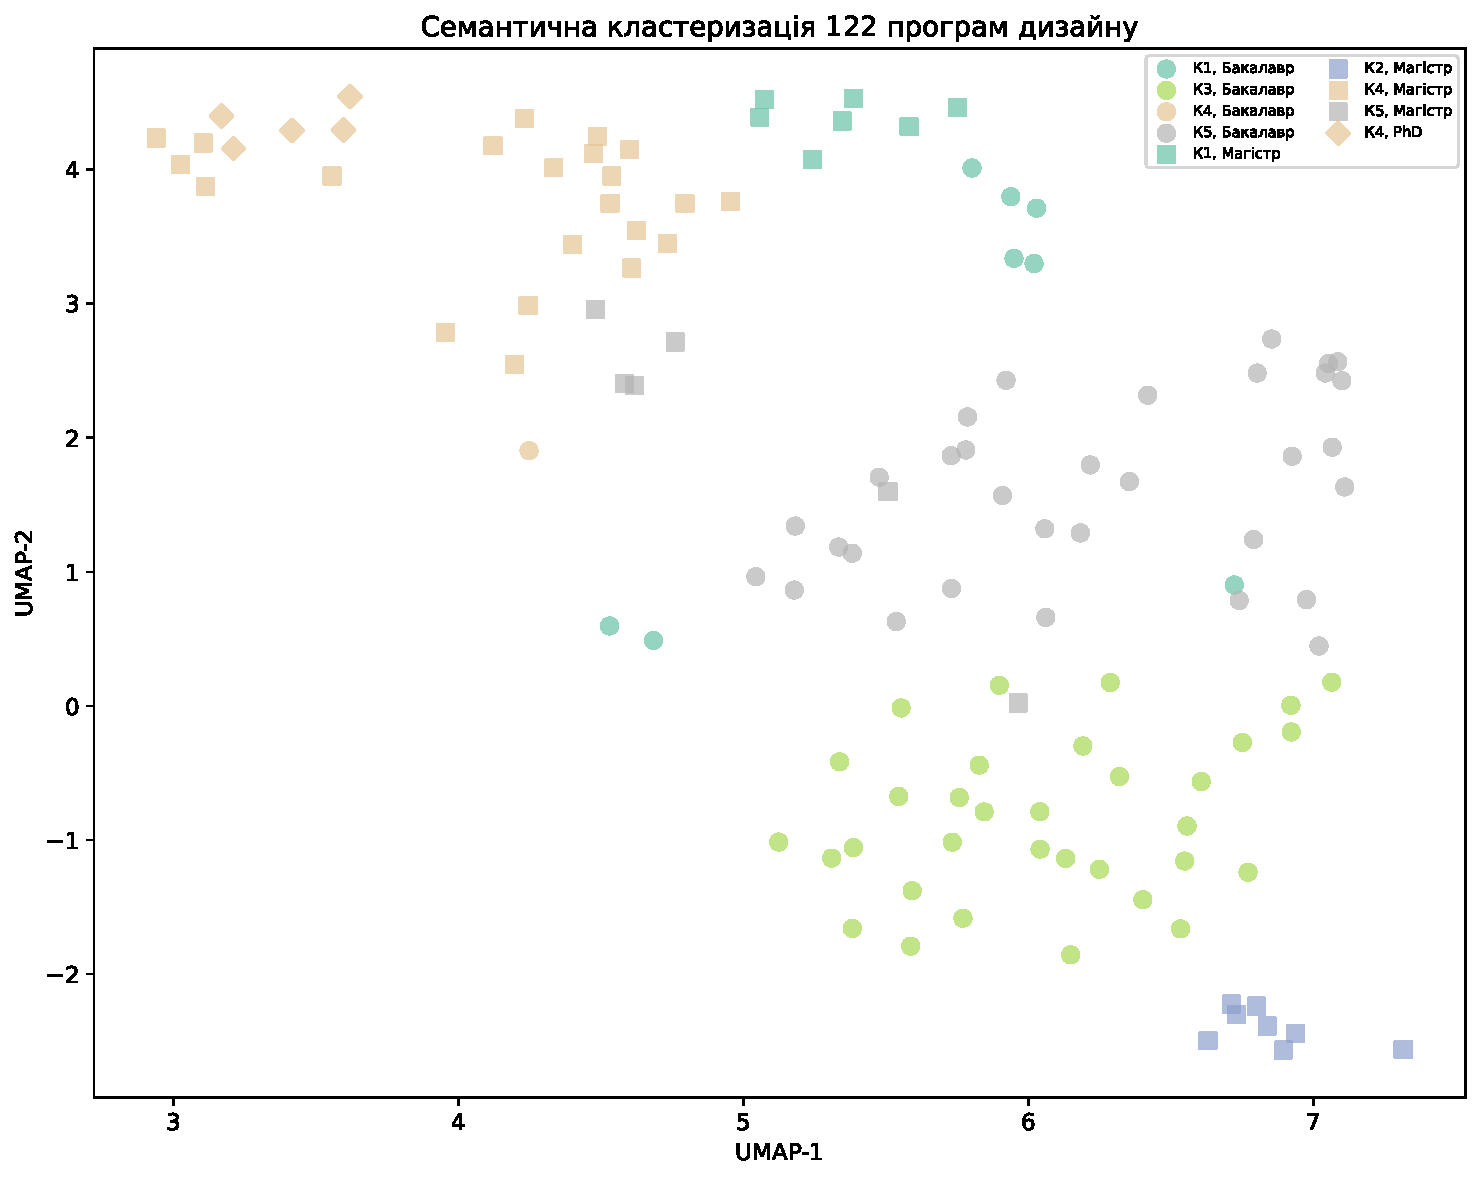
\includegraphics[width=0.85\textwidth]{figures/semantic_clusters.pdf}
\caption{Семантична кластеризація 122 програм дизайну (UMAP + K-Means)}\label{fig:semantic-clusters}
\end{figure}

Кластерна структура визначається переважно \textit{рівнем освіти} (бакалавр vs. магістр vs. PhD), а не змістовою спеціалізацією чи ступенем цифрової інтеграції. Жоден кластер не характеризується підвищеною концентрацією цифрових або ШІ-дисциплін. Висока однорідність ($\bar{s} = 0{,}772$) свідчить про обмежену диференціацію програм: більшість ЗВО пропонують подібний набір дисциплін, що ускладнює конкурентне позиціонування та оперативну адаптацію до вимог ринку.

\subsubsection{Аналіз ШІ/ІКК-розривів}\label{sssec:2.1.5}

Ключовим етапом аналізу є оцінка покриття ШІ-навичок та ІКК-компонентів у навчальних програмах. Для цього розроблено класифікатор, що зіставляє назви та описи дисциплін з переліком 20 ключових слів, пов'язаних із ШІ та цифровими технологіями.

\begin{table}[htbp]
\centering
\caption{Аналіз ШІ/ІКК-розривів у 122 програмах дизайну}\label{tab:gap-analysis}
\small
\begin{tabularx}{\textwidth}{@{}Xcc@{}}
\toprule
\textbf{Навичка / компонент} & \textbf{Покриття} & \textbf{Статус} \\
\midrule
\textit{Цифрові інструменти:} & & \\
\quad 3D-моделювання & 100\% & \checkmark \\
\quad Моушн-дизайн / Анімація & 100\% & \checkmark \\
\quad UX/UI дизайн & 100\% & \checkmark \\
\quad Інтерактивний / обчислювальний дизайн & 100\% & \checkmark \\
\quad 2D цифрові інструменти & 33,3\% & Частково \\
\quad Візуалізація даних & 33,3\% & Частково \\
\quad VR/AR дизайн & 33,3\% & Частково \\
\addlinespace
\textit{Компоненти ШІ:} & & \\
\quad \textbf{Основи ШІ} & \textbf{0\%} & \ding{55} \\
\quad \textbf{Генеративний ШІ та дизайн} & \textbf{0\%} & \ding{55} \\
\quad \textbf{Комп'ютерний зір} & \textbf{0\%} & \ding{55} \\
\addlinespace
\midrule
Загальне покриття цифрових інструментів & 71,4\% & Задовільно \\
\textbf{Загальне покриття ШІ} & \textbf{0\%} & Критично \\
\textbf{Загальне покриття} & \textbf{35,7\%} & Незадовільно \\
\bottomrule
\end{tabularx}
\end{table}

Результати аналізу розривів (таблиця~\ref{tab:gap-analysis}) є центральним емпіричним аргументом дисертації: при 71,4\% покритті традиційних цифрових інструментів, \textbf{жодна з 122 програм не містить дисциплін, спрямованих на основи ШІ, генеративний ШІ або комп'ютерний зір}. Загальне покриття ШІ-компонентів становить 0\%, а сукупне покриття ШІ-тематики~--- лише 35,7\%.

Цей розрив має безпосередній зв'язок із 4-компонентною структурою ІКК:
\begin{itemize}
    \item \textbf{Інформаційно-аналітичний компонент}: відсутність навчання роботі з ШІ-генерованою інформацією означає, що випускники не підготовлені до критичного оцінювання ШІ-виходів;
    \item \textbf{Технологічний компонент}: 0\% покриття ШІ-інструментів означає повну відсутність підготовки до використання Midjourney, DALL-E, Stable Diffusion та інших генеративних інструментів;
    \item \textbf{Комунікативний компонент}: без промпт-інженерії студенти не набувають здатності ефективно формулювати запити до генеративних моделей;
    \item \textbf{Рефлексивний компонент}: без тематики ШІ-етики та критичного аналізу ШІ в дизайні рефлексивний компонент залишається неповним.
\end{itemize}

\subsubsection{Висновки загальнонаціонального аналізу}\label{sssec:2.1.6}

Комплексний обчислювальний аналіз 122 українських програм дизайну виявив системну прогалину у формуванні ІКК: при задовільному покритті традиційних цифрових інструментів (71,4\%), ШІ-компоненти повністю відсутні (0\%). Мережевий аналіз підтвердив, що цифрові/ШІ-дисципліни не утворюють самостійного кластера у структурі програм. Тематичне моделювання (BERTopic, 134 теми) засвідчило домінування традиційних мистецьких та загальноосвітніх тем при повній відсутності тем, пов'язаних із ШІ. Семантична кластеризація ($\bar{s} = 0{,}772$) виявила 5 кластерів, диференційованих за рівнем освіти, а не за ступенем цифрової інтеграції, що засвідчує структурну однорідність програм. Ригідна структура навчальних планів (фактична відсутність вибіркових компонентів) ускладнює оперативне введення ШІ-тематики. Ці дані обґрунтовують необхідність системної трансформації навчальних програм, що є предметом розділу~3.
